\section{L'annalyse des donnée}
Une des premiere tache que j'ai effectuer a été que recaculer a partir des donnée brute recolter sur chaque slab la production mensuelle des differnet fosse de Somaïr. Pour cela, j'ai eu acess a la dataplatform de Orano qui est sur Dataiku. 

Dataiku est un platform concu pour symplifier et democratiser l'annalyse de donnée, Pour cela, il n'y a meme pas besoin d'écrire une ligne de code car Dataiku a des recette visuel. Pour ceux qui shouite aller plus loin, il est possible d'ecrire des recette en python ou en R. Pour effectuer mes analyse je me suis plutot appuyer sur les recette python qui exploite la librairie \href{https://pandas.pydata.org/}{pandas} et \href{https://numpy.org/}{numpy}.

Les donnée en provenance de la CanOp on d'abord besoin d'etre nettoyer car il y a parfois des probleme de mesure, des bug et l'operateur a la possibiliter de supprimer une mesure mais cette fonctionaliter est implementer de tel maniere que la mesure est toujours presente mais avec une valeur de -1. Il faut donc supprimer tout ces valeur. J'ai egalement eu une colonne ne contenant que des numero mais dont certaint etait sauver comme des string et d'autre comme des int.

J'ai ensuite pus etablire les teneur en uranium de chaque slab en utilisant la formule suivante:
\begin{equation}
    Teneur en uranium = \begin{cases}
        cps_{sonde_base}\footnote{cps sont des choc par seconde soit le nombre de photon qui sont rentre en colition avec le crystal} \times 0.0002 \\
        cps_{sonde_haut} \times 0.0011
    \end{cases}
\end{equation}
\begin{figure}
    \centering
    \begin{subfigure}{0.45\textwidth}
        \centering
        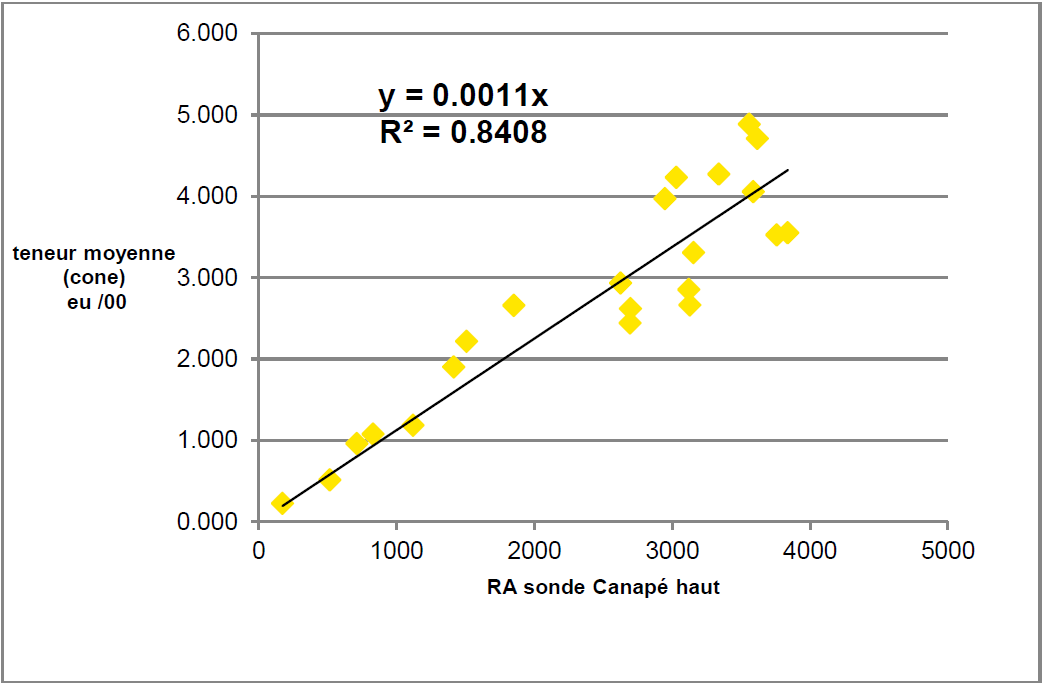
\includegraphics[width=\textwidth]{img/graph/Correlation_sonde_haute.png}
        \caption{Correlation pour la sonde haute}
        \label{fig:correlation_sonde_haute}
    \end{subfigure}
    \begin{subfigure}{0.45\textwidth}
        \centering
        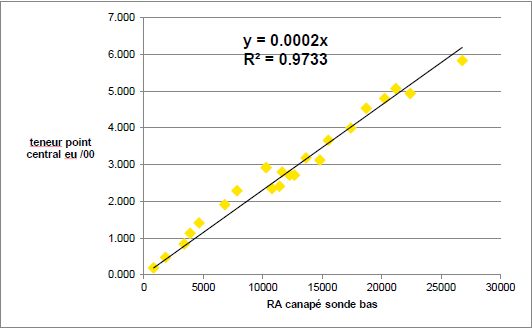
\includegraphics[width=\textwidth]{img/graph/Correlation_sonde_basse.png}
        \caption{Correlation pour la sonde basse}
        \label{fig:correlation_sonde_basse}
    \end{subfigure}
    \caption{Correlation entre la radiometrie et la teneur d'uranium pour les sonde haute et basse, Source: Compte-rendu de mission Orano, Réf. : IDF-CR-001714}
    \label{fig:correlation_sonde}
\end{figure}
Ces correlation on etait obtenu directement dans le fosse de Somaïr avec des mesure empirique (voir \cref{fig:correlation_sonde_haute,fig:}).
